% !TEX root = ../my-thesis.tex
%
\chapter{Motivation und Problemdefinition}\label{ch:Motivation und Problemdefinition}

\todo[inline,color=red!80]{Ob hier ein Section Header hinmuss oder nicht gilt zu klären, evtl. ist es schöner ohne? Oder einfach in 2 Teilen, pures Intro ohne und dann Automatisierung und so (siehe TODO unten) unter section\{Ausgangslage\}}
% \section{Ausgangslage}\label{ch:Ausgangslage}

Die Softwareentwicklung ist mehr denn je durch Anforderungen getrieben. Um dieser Notwendigkeit gerecht zu werden, wurde das Themengebiet des ''Requirements Engineering'' (RE) ins Leben gerufen, das bis zum heutigen Stand von einer starken Mehrheit der Entwickler als ''sehr wichtig'' empfunden wird.\cite{wangRoleRequirementsEngineering2014} Um der stets steigenden Menge an Anforderungen gerecht zu werden, ist die meistverbreitetste Methode, um Anforderungen darzustellen und zu dokumentieren, die ''User Story''\cite{wangRoleRequirementsEngineering2014}. Oft im originellen Format nach [...]\todo{cite} ist sie wie folgt definiert:

''As a \textlangle \textit{role}\textrangle, I want a \textlangle \textit{goal}\textrangle, [so that \textlangle \textit{benefit}\textrangle].''

Unter der Annahme, dass diese strukturiert und bewusst eingesetzt werden, stellen sie für viele Entwickler ein nützliches und produktivitätssteigerndes Werkzeug dar.\cite{lucassenUseEffectivenessUser2016}

Im Zeitalter von Large Language Models (LLMs) und agentischen Entwicklungsverfahren ist es so leicht wie nie zuvor, Quellcode aus Natürlichssprachigen Anforderungen zu erzeugen. Neben den bist dato stets steigenden Kapazitäten von LLMs diese Aufgabe (auch NL2Code genannt) zu lösen werden auch stets neue Benchmarks entworfen um diese Fähigkeiten gegenüber möglichst realistischen Bedienungen zu prüfen.\cite{jiangSurveyLargeLanguage2026} Dabei wird auffällig, dass Anforderungen oft, entgegen den Erkentnissen aus dem RE, in massiven Text-Korpusen integriert werden.

\todo[inline]{Weiterer Einstieg zur Automatisierung von Prozessen notewendig}

\section{Problemdefinition}\label{ch:Problemdefinition}

Die Frage die sich nun stellt ist ob die Verwendung von User-Stories für die Generierung von Quellcode nützlich ist. Doch hierfür muss zuerst der aktuelle Stand der Wissenschaft in Hinsicht auf die NL2Code Aufgabe analysiert und verstanden werden.

Hierbei ergeben sich mehrere Probleme, die es in dieser Arbeit zu betrachten gilt:

\begin{itemize}
    \item Vorhandene Arbeiten berichten ihre Ergebnisse oft unter eigenen Bedienungen (Beispielsweise Modelle, Hyperparameter, RAG-Strategien, Metriken und Benchmarks).
    \item Daher ist es oft nicht möglich diese Ergebnisse untereinander zu vergleichen.
    \item Aussagen zum Automatisierungsgrad sind generell heterogen und nicht vergleichbar.
\end{itemize}

Diese Gesichtspunkte machen es äußerst schwer die Fragen aus unser ursprünglichen Problemdefinition zu beantworten.

\section{Zielsetzung und Forschungsfragen}\label{ch:Zielsetzung und Forschungsfragen}

Ziel dieser Arbeit ist es, unter angesicht der oben genannten Probleme bestehende wissenschaftliche Arbeiten zu untersuchen und diese in Hinsicht auf die NL2Code Aufgabe einzuordnen und zu vergleichen. Hierzu wird der Stand der Grundlagen sowie aktuelle Lösungsansätze genauer betrachtet. Die Fragen und die Thematik stammen dabei von der Forschungsgruppe WSE, aufzufinden unter \cite{WSEResearchThema}. Die Arbeit fokussiert sich exlpizit auf folgende 2 Forschungsfragen:

\begin{description}
    \item[RQ1]\label{RQ1} \textbf{Wie kann aus Userstories passender funktionaler Quellcode und zugehöriger Text erzeugt werden?}
\end{description}

Es gilt zu untersuchen inwiefern LLMs in der Lage sind, User Stories (in natürlicher Sprache) in funktionsfähigen Quellcode zuzuwandeln. Folglich muss analysiert werden wie gut LLMs mit aktuellen Lösungsansätzen in der Lage sind die Anforderungen von User Stories zu interpretieren und darauf basierend vollständigen, syntaktisch korrekten funktionsfähigen Quellcode zu generieren.

Weiterhin soll in diesem Umfang auch geprüft werden, wie gut diese Modelle erklärende Texte, wie Kommentare oder API-Dokumentationen, automatisch erstellen können.

\begin{description}
    \item[RQ2]\label{RQ2} \textbf{Wie hoch ist der Automatisierungsgrad?}
\end{description}

Diese Frage analysiert den Grad der Autoamtisierung, der bei der Generierung von Quellcode aus Userstories erreicht werden kann. Es wird untersucht, inwieweit der Prozess vollständig automatisiert durchgeführt werden kann, ohne dass manuelle Eingriffe erforderlich sind. 

Dabei wird auch betrachtet, in welchen Phasen der Code-Generierung oder -Anpassung menschliche Eingriffe besonders wichtig sind und wo die Grenzen der LLM-basierten Automatisierung liegen.

\section{Erfolgskriterien und Abgrenzung}\label{ch:Erfolgskriterien und Abgrenzung}

Das Ziel dieser Arbeit ist es wie bereits beschrieben die Grundlagen zu erläutern und den aktuellen Stand zu vermitteln. In Hinsicht auf \rqref{RQ1} ergeben sich dadurch folgende Ziele für diese Arbeit:

\begin{enumerate}
    \item $N$ Lösungsansätze werden gegen $M$ Benchmarks evaluiert
    \item Die Bedienung für diese Evaluationen sind dokumentiert und für alle Durchläufe möglichst identisch
    \item Abweichungen zu publizierten Werten werden quantifiziert
\end{enumerate}

Hierzu muss erwähnt werden, dass es zum heutigen Stand keinen Benchmark gibt der tatsächlich mit User-Stories arbeitet. Daher kann die Frage \rqref{RQ1} nicht in Hinsicht auf Userstories analysiert werden, da dies außerhalb des Rahmens dieser Arbeit liegt. Für die Frage \rqref{RQ2} ergibt sich weiterhin folgendes Ziel:

\begin{enumerate}
    \item Es existiert ein Klassifikationsschema für existierende Arbeiten, welches deren Automatisierungsgrad erkennbar macht
\end{enumerate}

Die Beantwortung von \rqref{RQ2} erfolgt im Gegensatz zu \rqref{RQ1} nicht via einem Experiment. Die Einordnung erfolgt vie Klassifikation anhand der Arbeiten, da diese bereits ein umfangreiches Bild darstellen.

\section{Forschungsprozess / Vorgehen}\label{ch:Forschungsprozess / Vorgehen}

Das weitere Vorgehen in dieser Arbeit sieht folgender maßen aus: Zuerst sollen relevante Arbeiten aus dem Themenfeld betrachtet werden. Zu diesem Zweck erfolgt eine Literaturaufarbeitung, angelehnt and SLR-Verfahren (aber skaliert auf den Umfang dieser Arbeit). Daraus folgt die Ableitung von eigenen Experimenten, die den aktuellen Stand der Forschung darstellen und vergleichen sollen. Aufbauend auf dieser Ableitung folgt die Konzeption und folgliche Implementierung eines Orchestrators. Dieser soll die letzendliche Durchführung der Experimente ermöglichem. Schlussendlich folgt eine Darstellung der Ergebnisse und eine Einordnung.

\section{Aufbau der Arbeit}\label{ch:Aufbau der Arbeit}

\todo[inline]{Hier kommt die Überblick über die Struktur der Arbeit. TODO für das Ende!}

% \todo[inline]{1. Initiale Einleitung}

% \todo[inline]{2. Themen Überführung zu SWE}

% \todo[inline]{3. Von SWE zur modernen Verwendung von User Stories}

% \todo[inline]{4. Ableitung bisheriger Erkentnisse auf Code Generation via Agentic Systems}

% \subsection{Forschungsfragen}\label{research_questions}

% Im Rahmen dieser Arbeit soll der mögliche Einfluß von User Stories auf die Generation von Quellcode untersucht werden. Hierzu wird der Stand der Grundlagen sowie aktuelle Lösungsansätze genauer betrachtet. Dabei fokussiert sich die Arbeit exlpizit auf folgende 2 Forschungsfragen:

% \todo[inline]{Der Text zu den Forschungsfragen kommt von der \href{https://wse-research.org/thesis_topic/user-stories-to-code}{WSE Website} und ist legedlich leicht umformuliert. Ob das so okay ist gilt zu klären.}

% \begin{description}
%     \item[RQ1]\label{RQ1} \textbf{Wie kann aus Userstories passender funktionaler Quellcode und zugehöriger Text erzeugt werden?}
% \end{description}

% Es gilt zu untersuchen inwiefern LLMs in der Lage sind, User Stories (in natürlicher Sprache) in funktionsfähigen Quellcode zuzuwandeln. Folglich muss analysiert werden wie gut LLMs mit aktuellen Lösungsansätzen in der Lage sind die Anforderungen von User Stories zu interpretieren und darauf basierend vollständigen, syntaktisch korrekten funktionsfähigen Quellcode zu generieren.

% Weiterhin soll in diesem Umfang auch geprüft werden, wie gut diese Modelle erklärende Texte, wie Kommentare oder API-Dokumentationen, automatisch erstellen können.

% \begin{description}
%     \item[RQ2]\label{RQ2} \textbf{Wie hoch ist der Automatisierungsgrad?}
% \end{description}

% Diese Frage analysiert den Grad der Autoamtisierung, der bei der Generierung von Quellcode aus Userstories erreicht werden kann. Es wird untersucht, inwieweit der Prozess vollständig automatisiert durchgeführt werden kann, ohne dass manuelle Eingriffe erforderlich sind. 

% Dabei wird auch betrachtet, in welchen Phasen der Code-Generierung oder -Anpassung menschliche Eingriffe besonders wichtig sind und wo die Grenzen der LLM-basierten Automatisierung liegen.

% \todo[inline]{Hier kommt die Überblick über die Struktur der Arbeit. TODO für das Ende!}

% % \cleanchapterquote{The grand aim of all science [is] to cover the greatest number of empirical facts by logical deduction from the smallest possible number of hypotheses or axioms.}{Albert Einstein \cite{barnett2005universe}}{}


% % \begin{figure}[p]
% %     \centering
% %     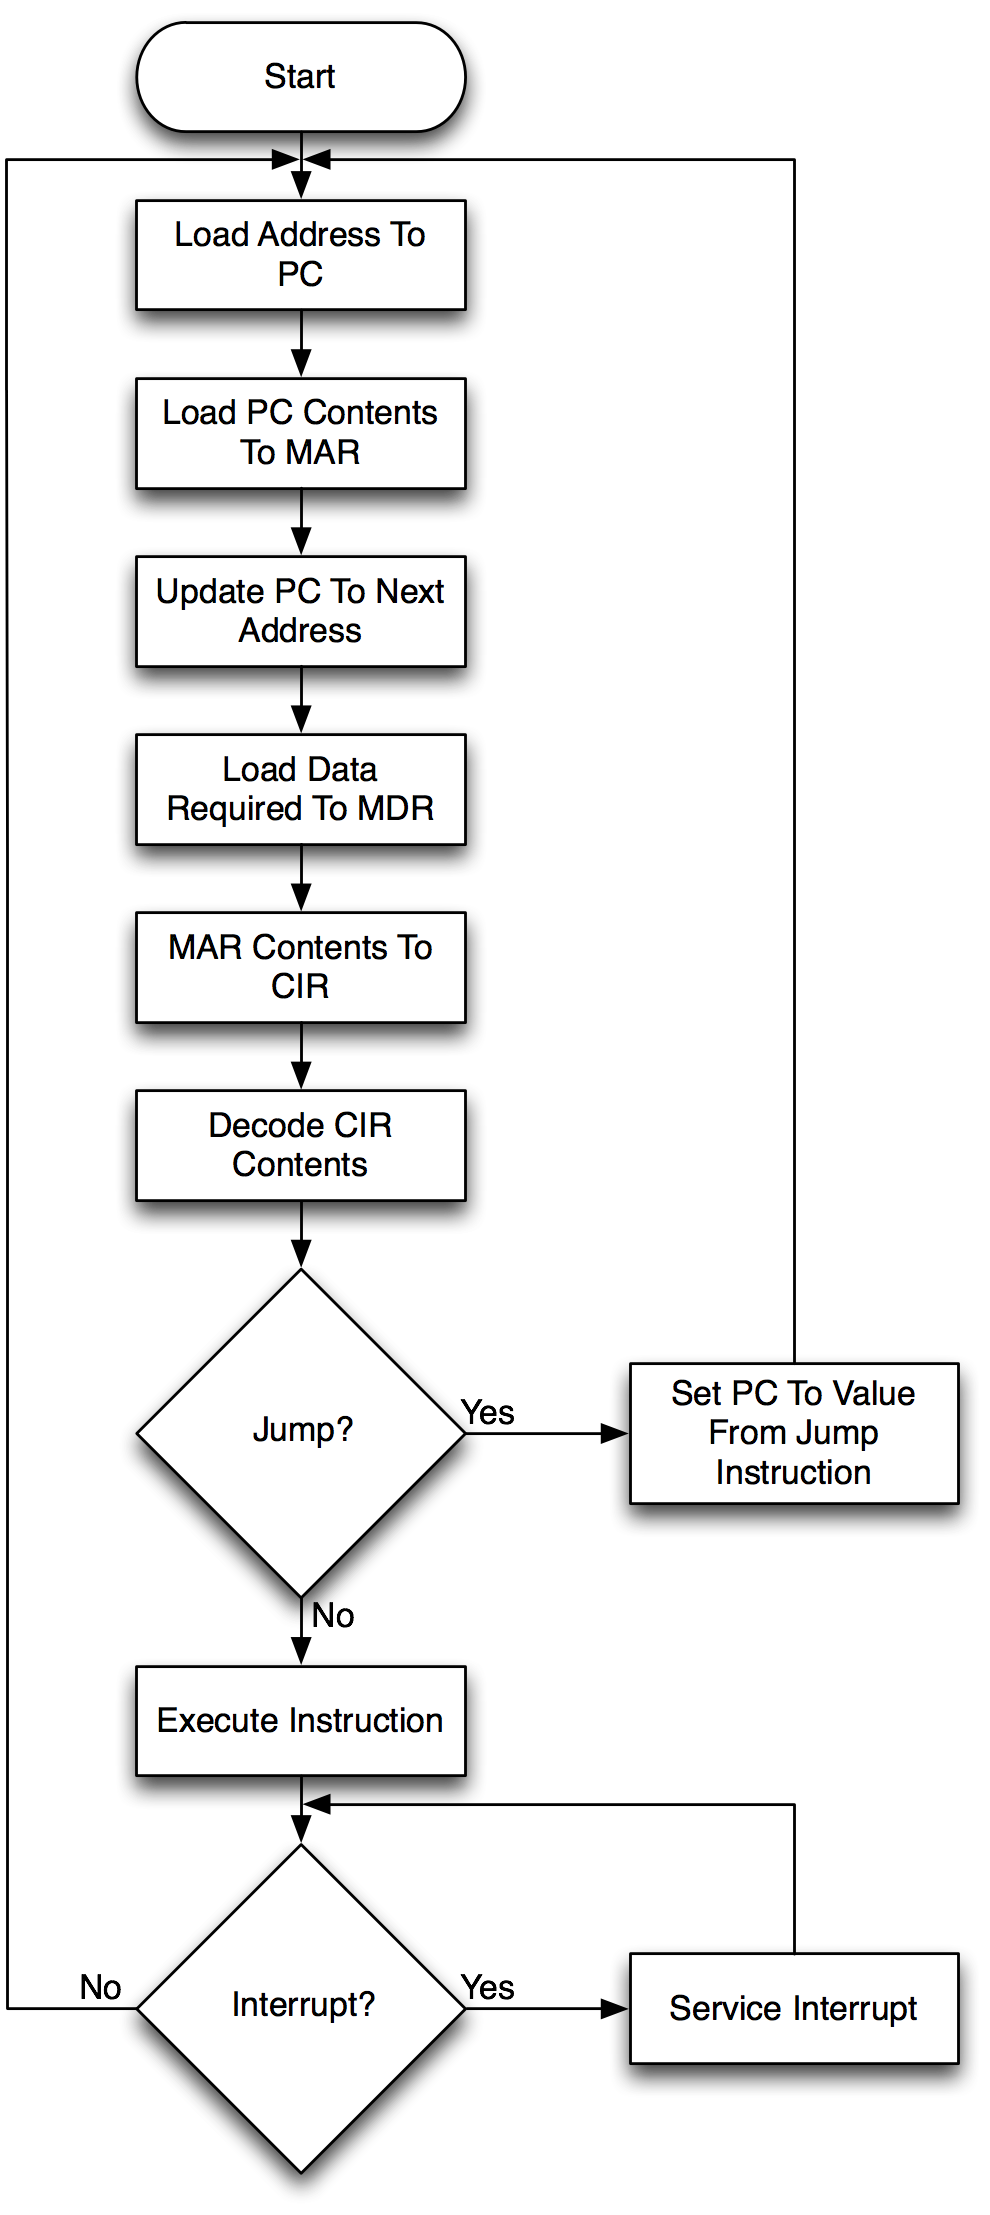
\includegraphics[height=\textheight]{images/Comp_fetch_execute_cycle.png}
% %     \caption{Every good research starts with a big picture describing the high-level research approach. \cite{WEB:flowchart_diagram}}
% %     \label{fig:big_picture}
% % \end{figure}

% % \lipsum[2-5] % remove 

% % \begin{figure}[t]
% %     \centering
% %     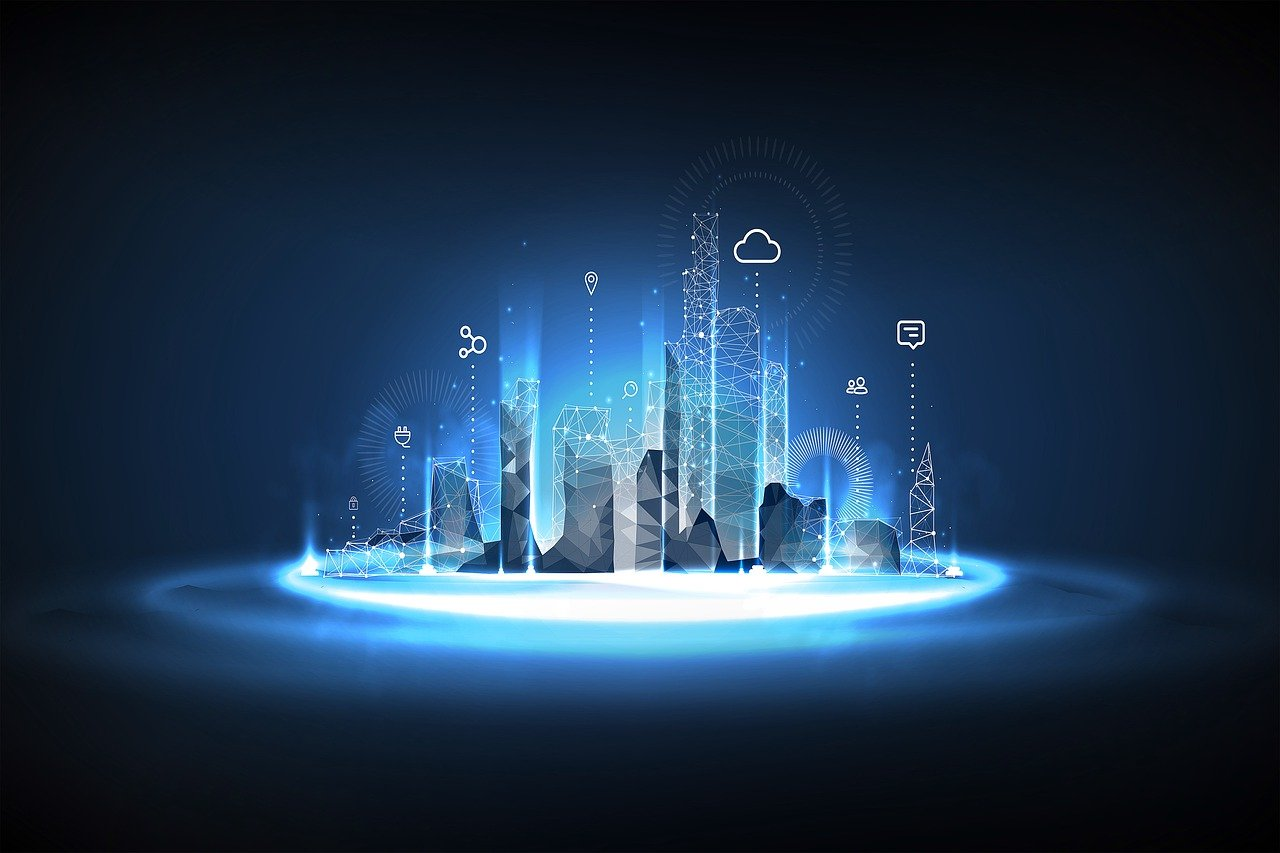
\includegraphics[width=.80\textwidth]{images/pixabay_technology-6701504_1280.jpg}
% %     \caption{Top-aligned image. \cite{PIXABAY:bild1}}
% %     \label{fig:image2}
% % \end{figure}

% % \lipsum[6-7] % remove 

% % \begin{description}
% %     \item[RQ1]\label{RQ1} ...
% %     \item[RQ2]\label{RQ2} ...
% %     \item[RQ3]\label{RQ3} ...
% %     \item[RQ4]\label{RQ4} ...
% % \end{description}

% % \lipsum[8-9] % remove 

% % \afterpage{ % Execute command after the next page break
% % \begin{landscape}
% % \begin{figure}
% %     \centering
% %     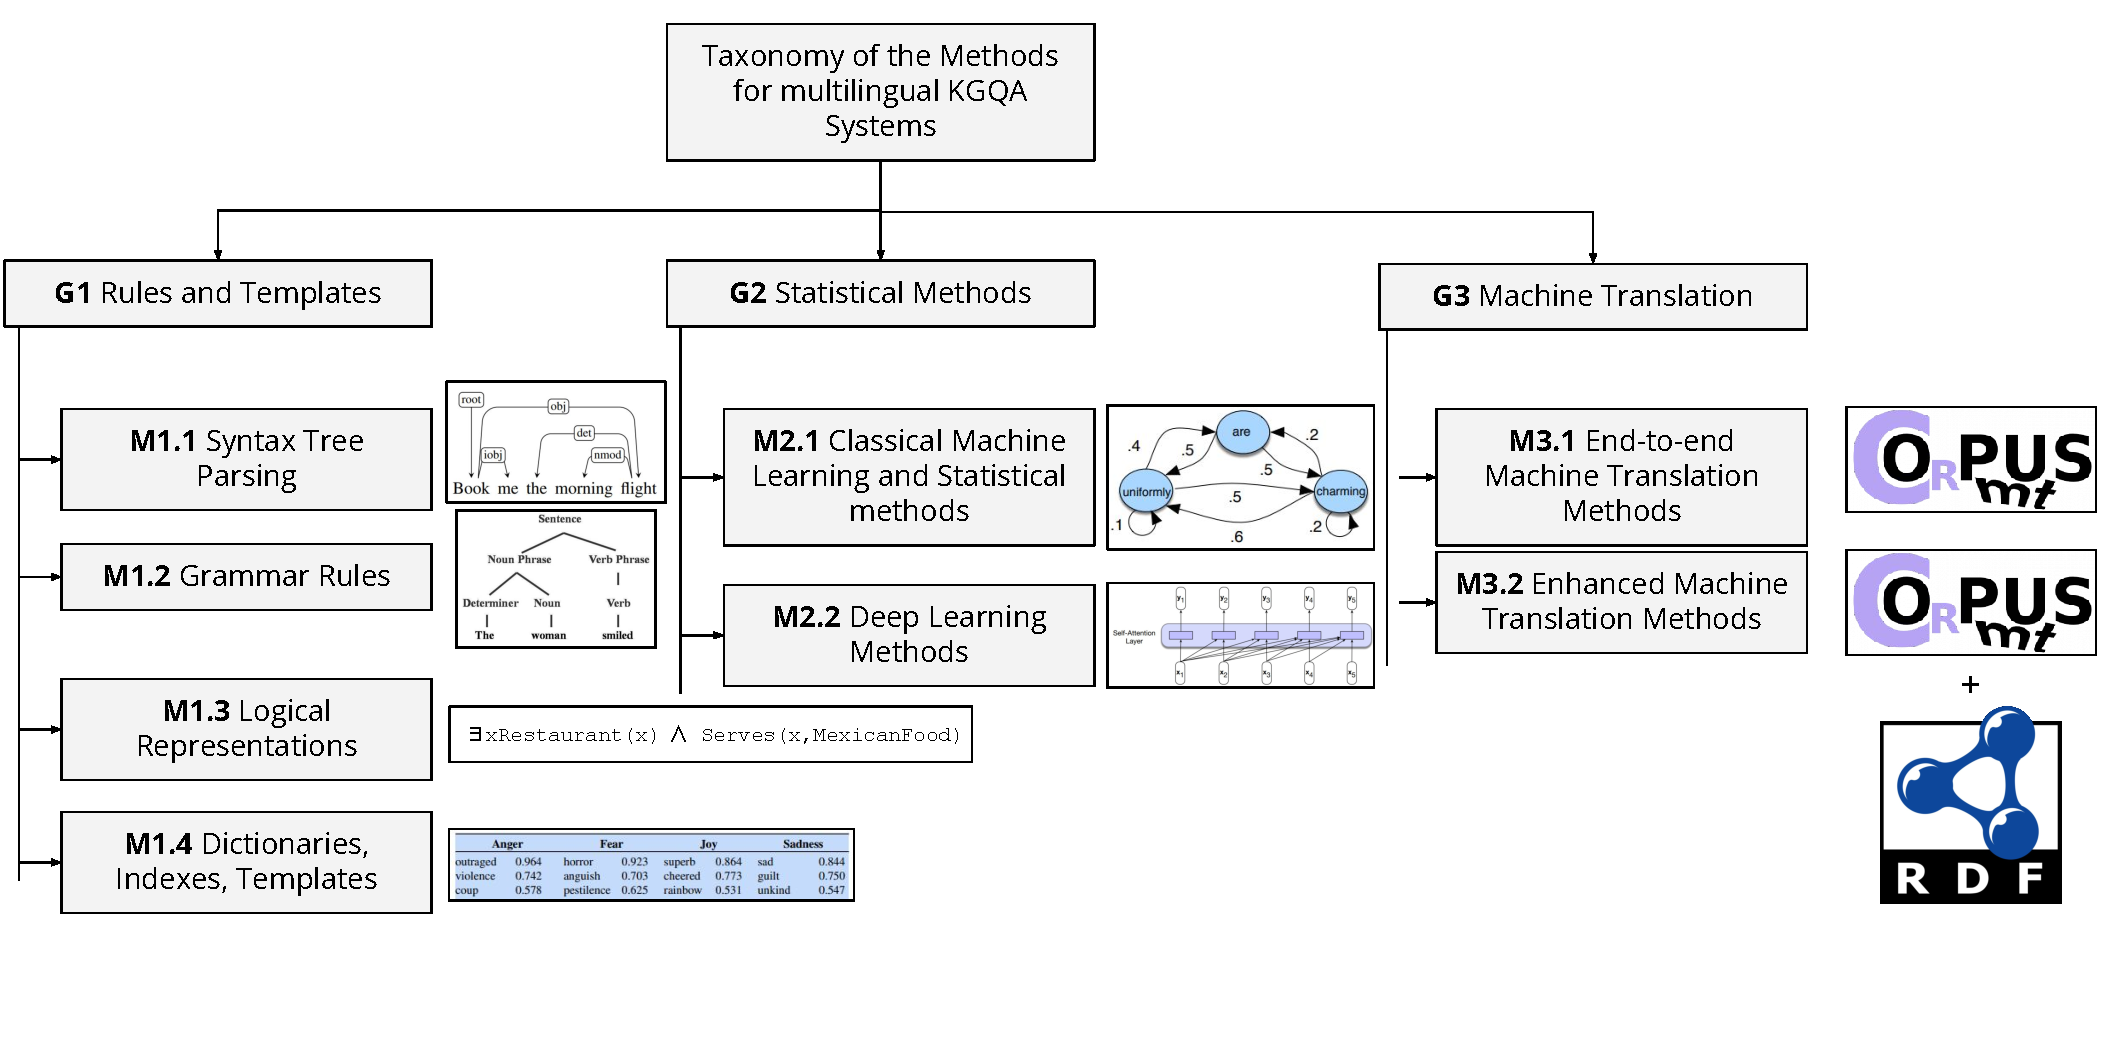
\includegraphics[width=\hsize]{gfx/taxonomy-multilingual-kgqa.pdf}
% %     \caption{An image in full landscape mode.}
% %     % source: https://docs.google.com/drawings/d/1M5NfSiLhNuRT3JuMr2WLTMpESCCnjup_Jok2EJlpzvI/edit?usp=sharing
% %     \label{fig:taxonomy}
% % \end{figure}
% % \end{landscape}
% % }

% % \lipsum[11-15] % remove 

% \controlquestions{
% \begin{enumerate}
%     \item Wurde eine Herleitung für das Thema vorgenommen (vom Allgemeinen, bis zum speziellen Themenbereich)?
%     \item Ist erkennbar, warum diese Arbeit besonders wichtig ist?
%     \item Wurde mindestens eine Forschungsfrage nachvollziehbar hergeleitet?
%     \item Wurde mindestens eine Forschungsfrage präzise formuliert?
%     \item Wurde der Ablauf (Forschungsprozess) der Arbeit dargestellt?
%     \item Wurde das messbare Erfolgskriterium benannt?
%     \item Wurde im letzten Abschnitt ein Überblick über die Struktur der Arbeit gegeben?
% \end{enumerate}
% }

